\documentclass{proc}

\usepackage[margin=1in]{geometry}   
\usepackage{multirow}
\usepackage{graphicx}
\usepackage{caption}
\usepackage{subcaption}

\graphicspath{{graphs/}}

\title{More tables and graphics}
\author{Bruno C. Messias}
\date{}

\begin{document}

\maketitle

\section{Introduction}

Look more about tables and graphics.

\subsection{More on Tables}


Table~\ref{tab}

\begin{table}[htbp]
    \caption{table}
    \centering
    \begin{tabular}{|c|c|p{3cm}|}
        \hline
        CS101 & Java & Programming with Java \\
        CS201 & Languages & Programming Languages Principles \\
        Cs301 & Compliers & Principles of Compilers \\
        \hline
    \end{tabular}
    \label{tab}
\end{table}

\begin{table}[htbp]
	\centering
	\caption{Spanning}
	\begin{tabular}{|c|c|c|}
		\hline
        & \multicolumn{2}{c|}{Ranges} \\
        & X & Y \\
        \hline
        \multirow{3}{*}{HOT} & 7 & 9 \\
        & 5 & 8 \\
        & 6 & 7 \\
        \hline
        \multirow{3}{*}{COLD} & 7 & 9 \\
        & 2 & 9 \\
        & 3 & 5 \\
        \hline
	\end{tabular}
\end{table}

\subsection{More on Graphics}

Both of my figures are in the the folder graphs, look the Figure \ref{graph} and Figure \ref{graph2} and Figure \ref{subs}.


\begin{figure}[htbp]
    \centering
    \begin{subfigure}[b]{0.2\textwidth}
        \centering
        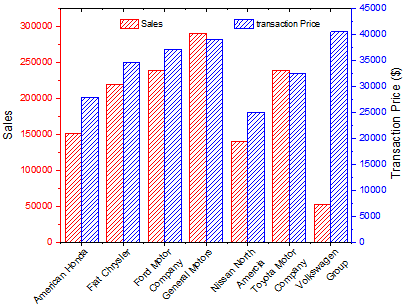
\includegraphics[scale=.2]{DoubleY_Column.png}
        \caption{Beginning}
        \label{graph}
    \end{subfigure}%

    \begin{subfigure}[b]{0.2\textwidth}
        \centering
        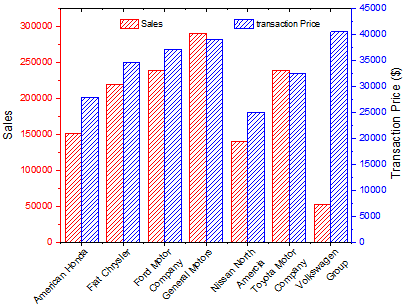
\includegraphics[scale=.2]{DoubleY_Column.png}
        \caption{End}
        \label{graph2}
    \end{subfigure}%

    \caption{The Process}
    \label{subs}
\end{figure}

\subsection{}


\section{Conclusion}




\end{document}